\section{Study 1: the paired effect of retaining assistant replies}
\label{sec:study1}

\subsection{Design}

\paragraph{Tasks and sample.}
We used the public math subset of Lost in Conversation \citep{laban2025lost}:
103 GSM8K-derived problems \citep{cobbe2021training}, each split into ordered
information shards, with one shard revealed per turn. Before any model was
queried, an input audit excluded 17 tasks. Eleven duplicated inputs of our
earlier experiments, eight appeared to change meaning when sharded, and two
belonged to both groups. A deterministic hash-based procedure that used no model
output then drew \nTasks{} science tasks with 4--9 shards (median 6) and four
disjoint integration tasks. The integration stage checked only transport,
resumption, parsing, scorers and plotting, and its outcomes could not alter the
sample or the analysis.

\paragraph{Models and arms.}
Three models were accessed through an academic gateway: GPT-4o-mini
\citep{openai2024gpt4o}, Llama-4 Scout and Mistral-7B \citep{jiang2023mistral}.
At every turn $t$, each model answered twice from identical user shards
$1,\dots,t$: in the dialogue-history arm, its own earlier primary replies were
interleaved; in the fresh-prefix arm, they were omitted
(Section~\ref{sec:framework}). The system prompt asked the model to solve
incrementally from the information given and stated that earlier assistant
replies might be wrong. Every reply had to end with exactly one line,
\texttt{FINAL\_ANSWER: <number>} once the answer was determined, or
\texttt{STATUS: NEED\_MORE\_INFORMATION} otherwise. Each cell received
$K=\Krep{}$ same-context samples and $L=\Lpar{}$ replies to frozen rewordings
of the instruction, at temperature \Ktemp{} and a \maxTok{}-token ceiling. Only
the primary sample entered later history.

The acquisition produced \nRecords{} successful calls, none truncated. Six
Mistral-7B primaries were empty despite a successful status. They were kept as
invalid, never retried, and represented in later history by a fixed
placeholder. Integration showed that the original strict final-line parser
rejected many replies that did contain an explicit marker. Before the science
run we therefore froze a parser that still requires the marker but tolerates
numbering, units and minor variants. Strict scores are preserved alongside.

\paragraph{Frozen analysis.}
The primary endpoint was paired final-turn success, tested by exact McNemar
tests \citep{mcnemar1947note} with task-bootstrap 95\% confidence intervals
(\nPermutations{} resamples; \citealp{efron1979bootstrap}) and Holm correction
across the three models \citep{holm1979simple}. Before the last shard, most
tasks have no determined answer, so CQ, RS and ES are structurally unobservable
there. The pre-final warning candidates were therefore CS, LS and SS. Each was
tested by a task-clustered partial correlation with final failure in the
dialogue arm, adjusting for model, turn, the revealed-information fraction and
log context length, with one-sided task-clustered permutation tests and Holm
correction across the three metrics. CRL was frozen as an auxiliary measure;
its target was a positive final readiness gap, in which the fresh prefix
attempts an answer while the history arm remains unresolved.

\subsection{Results}

\paragraph{Retaining assistant replies lowers final success (confirmatory).}
Table~\ref{tab:s1primary} and Figure~\ref{fig:s1} report the primary endpoint.
Final success fell from \freshGpt{} in the fresh prefix to \dialGpt{} under
dialogue history for GPT-4o-mini (difference \diffGpt{}, 95\% CI \ciGpt{},
Holm $p=\pHolmGpt$) and from \freshMistral{} to \dialMistral{} for Mistral-7B
(\diffMistral{}, CI \ciMistral{}, Holm $p=\pHolmMistral$). Llama-4 Scout
showed the same direction (\diffLlama{}, CI \ciLlama{}) without confirmatory
significance (Holm $p=\pHolmLlama$). Discordant tasks were strongly
asymmetric across models: in \nFreshOnly{} tasks only the fresh prefix
succeeded, in \nDialOnly{} only the history arm did. Restricting the analysis
to tasks whose final replies were format-valid in both arms left the GPT-4o-mini
and Mistral-7B effects intact (supplementary Table~S3).

The Mistral-7B case shows how such a harm can arise. With its own replies in
context, the model tended to remain in an explicit ``need more information''
state at the last turn. Given the same information without those replies, it
attempted an answer. The history did not merely add noise to the computation; it
changed whether the model regarded the task as solvable.

\begin{table}[t]
\centering
\caption{Study 1 paired final-turn success over \nTasks{} tasks per model.
F/D: number of tasks in which only the fresh prefix, or only the dialogue
history, succeeded. $p$: exact McNemar test.}
\label{tab:s1primary}
\small
\resizebox{\linewidth}{!}{%
\begin{tabular}{lcccccc}
\toprule
Model & Dialogue history & Fresh prefix & Diff.\ [95\% CI] & F/D & $p$ & $p_{\text{Holm}}$\\
\midrule
\inputtable{generated/table_primary.tex}
\bottomrule
\end{tabular}
}
\end{table}

\begin{figure}[t]
\centering
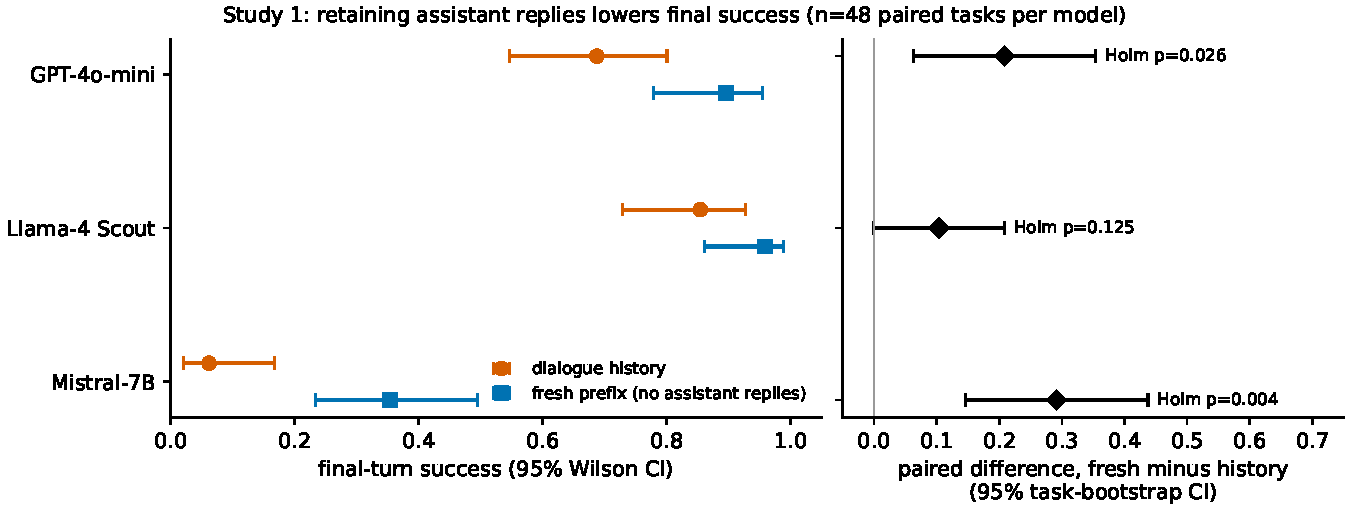
\includegraphics[width=\linewidth]{study1_paired.pdf}
\caption{Study 1 primary endpoint ($n=\nTasks{}$ paired tasks per model).
Left: final-turn success in each arm with 95\% Wilson intervals
\citep{wilson1927probable}. Right: paired difference, fresh prefix minus
dialogue history, with 95\% task-bootstrap intervals and Holm-adjusted McNemar
$p$-values.}
\label{fig:s1}
\end{figure}

\paragraph{The measurable quality metrics do not warn (confirmatory).}
None of CS, LS and SS carried information about final failure beyond turn,
revealed information and context length (Table~\ref{tab:s1rqeval}). All
partial correlations were close to zero, and every Holm-adjusted $p$-value was
1.0. CS had little support, because before the final shard most samples did
not commit to an answer.

\begin{table}[t]
\centering
\caption{Study 1 pre-final metrics as predictors of final failure under
dialogue history. Turns: scored pre-final turns; units: model--task units;
$r_{\text{partial}}$: task-clustered partial correlation; $p$: one-sided
task-clustered permutation test.}
\label{tab:s1rqeval}
\small
\begin{tabular}{lcccccc}
\toprule
Metric & Turns & Units & Tasks & $r_{\text{partial}}$ & $p$ & $p_{\text{Holm}}$\\
\midrule
\inputtable{generated/table_rqeval.tex}
\bottomrule
\end{tabular}
\end{table}

\paragraph{The paired readiness measure reduces to persistence.}
CRL discriminated its frozen target modestly (pooled model-stratified AUROC
\crlAuroc{}, task-clustered permutation $p=\crlP$, bootstrap CI \crlCi{}),
driven by GPT-4o-mini and Mistral-7B (supplementary Table~S2). A post-hoc check
compared CRL with simple baselines. The last pre-final readiness gap alone did
better (AUROC \crlLastGapAuroc{}, $p=\crlLastGapP$), and within strata of that
gap CRL carried no further information (AUROC \crlCondAuroc{},
$p=\crlCondP$). CRL therefore measures the persistence of an unresolved state
rather than anticipating failure beyond the current state. When the target was
replaced, post hoc, by accuracy loss (fresh prefix correct, history wrong), the
association was borderline (AUROC \robAllAuroc{}, $p=\robAllP$) and came from
Mistral-7B alone. Even a paired, counterfactual measure thus did not anticipate
the failure; it registered it once the history arm had already fallen behind.
